% !TeX spellcheck = english
% !TEX root = thesis.tex
\section{Methods}
\label{ch:Exp}

    \subsection{Fabrication of Crystalline Silicon Nanoparticles by Femtosecond Laser Ablation}
    \label{sec:Ablation}
            The first part of the project was to develop a new, simple, method of fabricating crystalline dielectric
        nanoparticles. The idea was to use controlled laser ablation~--- a very simple technique~--- to produce the particles.
        Previous work on the topic\cite{kuznetsov2012magnetic, zywietz2014laser} has shown that it is possible to fabricate single particles
        of a certain size.

            We ended up developing two different methods to fabricate crystalline nanoparticles~--- direct laser writing of crystalline
        nanoparticles out of a thin film of amorphous silicon (adapted from a method used for plasmonic nanoparticles\cite{makarov2016controllable,
        dmitriev2016direct}), and a forward transfer of nanoparticles by single femtosecond laser pulses
        from a transparent substrate with a a thin film of amorphous silicon to an arbitrary acceptor substrate. The second method is
        similar to the the one presented in \cite{zywietz2014laser}, but does not require any additional annealing steps to achieve
        nanoparticle crystallinity and is not limited to transparent acceptor substrates.

        \begin{figure}[h!]
                \begin{center}
                    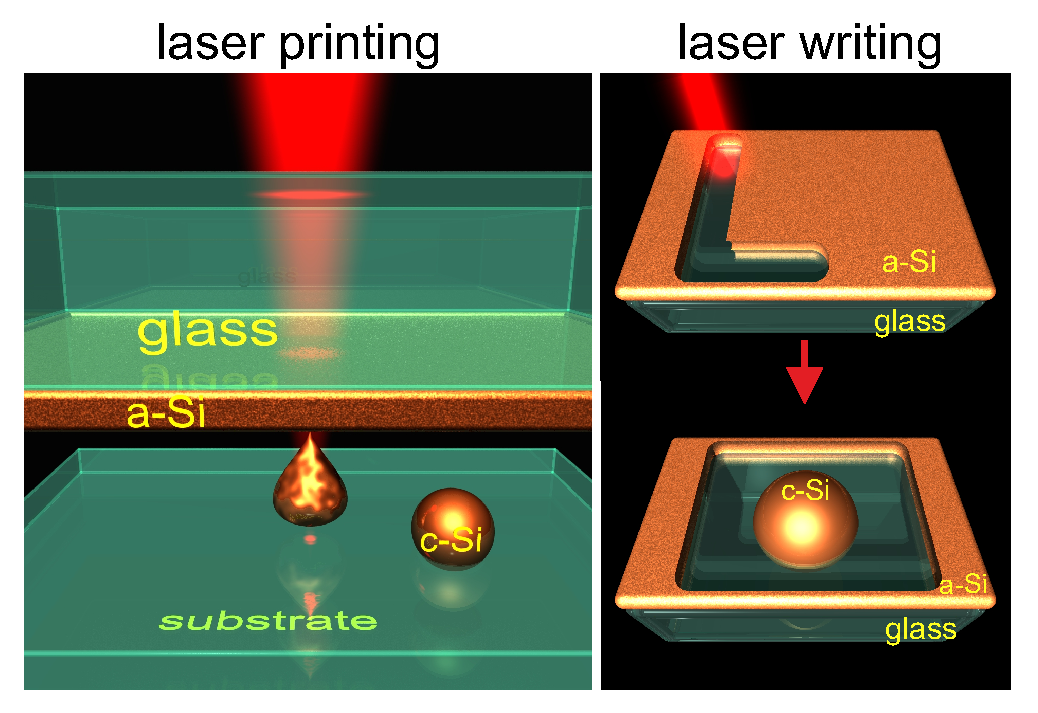
\includegraphics[width=0.5\textwidth]{figs/methods/LaserPrinting.eps}
                \end{center}
                \caption{Geometry of laser-ablation based fabrication methods of crystalline nanoparticles from amorphous
                            thin films.}
                \label{fig:LaserPrinting}
        \end{figure}

        \subsubsection{Laser Transfer of Crystalline Dielectric Particles}
                Single laser pulses were selected by a Pockels cell-based pulse picker (also Avesta Project),
            focused by an oil immersion microscope objective (Olympus $100\times$)
            with a numerical aperture of $\mathit{NA}=1.4$. According to the relation $\emph{d}\approx 1.22\lambda/\mathit{NA}$, the estimated
            diameter of the beam's focal spot size was $d=0.7~\si{\upmu m}$, which was close to the value measured by a method based on
            the dependence of the laser-damaged area on incident laser energy ($0.68~\si{\upmu m}$)~\cite{liu1982simple}.
            The nanoparticles were fabricated from an $80~\si{nm}$ thick a-Si:H film deposited on a fused silica substrate by
            plasma enhanced chemical vapor deposition from a SiH$_{3}$ precursor gas.

                The nanoparticles were fabricated by single laser pulses (from a previously undamaged surface of the a-Si:H film) in a
            forward-transfer geometry, where the receiving substrate is placed under the film with a spacing
            of $\sim 50~\si{\upmu m}$ (figure~\ref{fig:LaserPrinting}(a)). This geometry has an advantage over the back-transfer geometry
            used in \cite{zywietz2014laser}, because of the possibility of transferring nanoparticles onto a wide variety of substrates,
            including opaque and structured samples.

                The silicon nanoparticles were printed at laser energies in the range of $0.5-1.2~\si{nJ}$, providing fluencies in
            the range of $0.12-0.16~\si{J/cm^{2}}$. The fabricated nanoparticles were almost spherical in shape(figure~\ref{fig:Crystallinity}(b))
            and their diameters lie in the range of $50-200~\si{nm}$, depending on the fluence.

        \subsubsection{Laser Writing of Dielectric Particles}
                The direct laser writing of crystalline Si nanoparticles was carried out from an initially amorphous a-Si:H film.
            The process consists of using a train of femtosecond pulses to cut patches out of the a-Si thin film\cite{makarov2016controllable,
            dmitriev2016direct}. A laser fluence $F\approx100~\si{mJ/cm^{2}}$ provides film heating close to the melting point even in a
            single shot regime, while a pulse train with a $12.5~\si{ns}$ delay between pulses leads to the temperature accumulation
            and exceeding of the ablation threshold. The heat transferring from the ablated area to the surrounding film is accumulated
            much stronger in the cut patches, which are thermally isolated from the rest of the film.
            These micro-patches are unstable at high temperatures and undergo dewetting to a certain number of similar
            nanoparticles~\cite{thompson2012solid}.

    \clearpage
    \subsection{Optical Measurements}
            All of the optical characterization measurements were carried out on a multifunctional setup, depicted in
            Fig.~\ref{fig:expSetup}. The setup allowed us to measure optical signals from single nanoparticles, provided that
            there was at least $1\mu$ m between the nanoparticle and its nearest neighbors. The XYZ-stage used for the
            positioning of the particles had $100$nm precision, giving enough control to position a single nanoparticle into
            the center of the excitation beam.

            The scattered light was collected from the top by an objective (Mitutoyo M Plan APO NIR, 100x, NA=0.7),
            sent to a Horiba LabRam HR spectrometer and projected onto a thermoelectrically cooled charge-coupled device
            (CCD, Andor DU 420A--OE 325) with a 150-g/mm diffraction grating. The spectrometer gave us a spectral resolution
            of around $1$nm.

            \begin{figure}[!ht]
                    \begin{center}
                        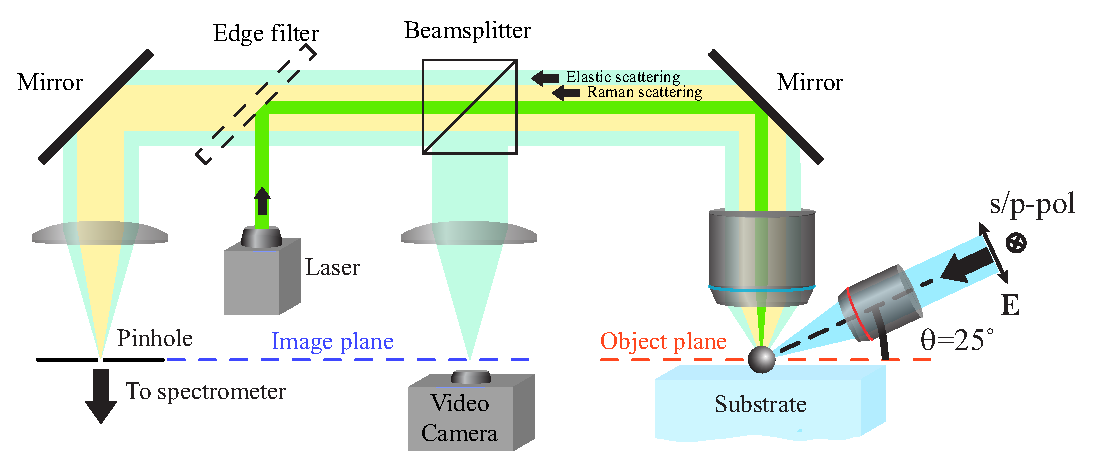
\includegraphics[width=0.9\textwidth]{figs/methods/expSetup2.eps}
                    \end{center}
                    \caption{Schematic of the experimental setup used for all of the optical measurements.}
                    \label{fig:expSetup}
            \end{figure}

        \subsubsection{Polarization-Resolved Dark-field Spectroscopy of Single Nanoparticles}
            \label{sec:Darkfield}
                For the dark-field scattering experiments, the nanoparticles were excited at an oblique angle of incidence
            (65 degrees to the surface normal) by linearly polarized light from a halogen lamp (HL--2000--FHSA)
            through a weakly-focusing objective (Mitutoyo M Plan Apo NIR, 10x, NA=0.28). The polarization allowed us to
            selectively excite different modes in the nanoparticles\cite{permyakov2015probing}.

            \begin{figure}[!ht]
                    \begin{center}
                        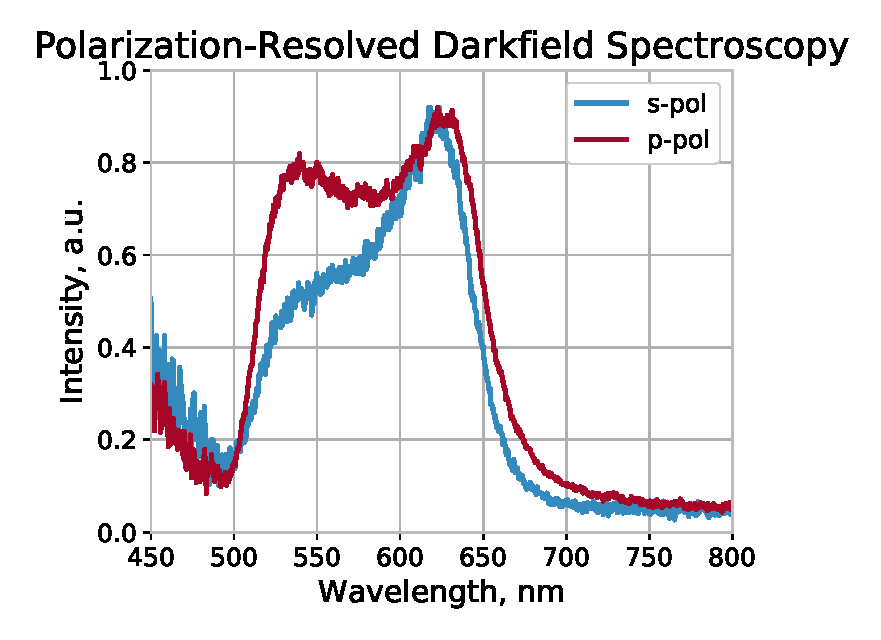
\includegraphics[width=0.6\textwidth]{figs/methods/DF/id_52780.eps}
                    \end{center}
                    \caption{Different Mie-type resonances excited by different polarizations of incident light.}
                    \label{fig:PolarizedDF}
            \end{figure}

        \subsubsection{Raman Spectroscopy of Single Nanoparticles}
        \label{sec:Raman}
                For the Raman scattering experiments, the nanoparticles were excited by one of two laser sources: a $632.8$nm HeNe laser
            or a $532$nm Nd:YAG laser, through the same channel that was used to collect the scattered light. A lowpass filter was used
            to filter out the excitation wavelength and leave only the Stokes-shifted inelastically scattered light.

    \subsection{Analytical Model of Raman Signal Enhancement by Mie resonances of Nanoparticles}
        \label{sec:Theory}
            This derivation is based on the derivation from \cite{dmitriev2016resonant}.

            To describe the enhancement of Raman scattering and analyze the role of the electric and magnetic
        Mie resonances of a silicon nanoparticle, we employ the rigorous Green tensor approach. Ideologically,
        our theoretical approach is based on earlier related studies~\cite{canccado2014theory, murphy1983enhanced}.

        In this framework, we first determine the spatial field distribution $\mathbf{E}_{exc}(\mathbf{r})$
        inside the nanoparticle at the excitation frequency created by an external source. Assuming that a
        spherical nanoparticle in free space is illuminated by a plane wave, we represent the normalized
        electric field inside the nanoparticle as a series of vector spherical harmonics~\cite{bohren1983absorption}:
        %
        \begin{align}
            \mathbf{E}_{exc}(\mathbf{r})=\sum\nolimits_{n=1}^\infty E_n \left(c_n\mathbf{M}_{o1n}^{(1)}(\mathbf{r}) -
            i{d_n}\mathbf{N}_{e1n}^{(1)}(\mathbf{r})\right) ,
            \label{eq1}
        \end{align}
        %
        where $c_n$ and $d_n$ are the Mie coefficients, ${{\mathbf{M}}_{o1n}^{(1)}}$ and ${{\mathbf{N}}_{e1n}^{(1)}}$ are
        the orthogonal vectorial spherical harmonics, and ${E_n} = {i^n}(2n + 1)/[n(n + 1)]$. The excitation field distribution
        at each point inside the medium defines the Raman polarization oscillating at the Stokes frequency $\omega_S$ according to
        %
        \begin{align}
            {{\bf{P}}_s}\left( {\bf{r}} \right) = {\chi _s}\hat \alpha_j \left( {\bf{r}} \right){{\bf{E}}_{exc}}\left( {\bf{r}} \right),
            \label{eq2}
        \end{align}
        %
        where $\chi_s$ is the scalar Raman susceptibility, and $\hat \alpha_j$ is the Raman polarizability tensor representing
        the threefold degenerate transverse optical (TO) phonon mode excitation~\cite{ralston1970spontaneous, peter2010fundamentals}.
        Induced Raman polarization, in turn, produces an electromagnetic field at the observation point
        $\mathbf{r}_0$ given by $\mathbf{E}_s(\mathbf{r}_0) = (\omega_s^2/c^2)\int\limits_V {{{\hat G}_s}\left( {{{\mathbf{r}}_0},{\mathbf{r}}} \right){{\mathbf{P}}_s}\left( {\mathbf{r}} \right){d^3}{\mathbf{r}}}$,
        where  ${\hat G_s}\left( {{{\mathbf{r}}_0},{\mathbf{r}}} \right)$ is the Green tensor at the Stokes frequency accounting
        for the Si nanoparticle and integration is carried out over the nanoparticle volume $V$. Finally, the collected signal at
        the point $\mathbf{r}_0$ is presented in the form:
        %
        \begin{align} %Final collected signal
            S\left( {{{\mathbf{r}}_0}} \right)
                =  \sum\limits_j {\left \langle{{\mathbf{E}}_s^*\left( {{{\mathbf{r}}_0}} \right){{\mathbf{E}}_s}\left( {{{\mathbf{r}}_0}} \right)} \right\rangle}
                = \sum\limits_j {\frac{{\omega _s^4}}{{{c^4}}}\iint\limits_V {{d^3}{{\mathbf{r}}_1}{d^3}{{\mathbf{r}}_2}\left\langle {\hat G_s^*\left( {{{\mathbf{r}}_0},{{\mathbf{r}}_1}} \right){\mathbf{P}}_s^*\left( {{{\mathbf{r}}_1}} \right){{\hat G}_s}\left( {{{\mathbf{r}}_0},{{\mathbf{r}}_2}} \right){{\mathbf{P}}_s}\left( {{{\mathbf{r}}_2}} \right)} \right\rangle }}  \\
                = \sum\limits_j {\frac{{\omega _s^4}}{{{c^4}}}\iint\limits_V {{d^3}{{\mathbf{r}}_1}{d^3}{{\mathbf{r}}_2}\hat G_s^*\left( {{{\mathbf{r}}_0},{{\mathbf{r}}_1}} \right){\mathbf{E}}_{exc}^*\left( {{{\mathbf{r}}_1}} \right){{\hat G}_s}\left( {{{\mathbf{r}}_0},{{\mathbf{r}}_2}} \right){{\mathbf{E}}_{exc}}\left( {{{\mathbf{r}}_2}} \right)\chi _s^2\left\langle {\hat \alpha _j^*\left( {{{\mathbf{r}}_1}} \right) \otimes {{\hat \alpha }_j}\left( {{{\mathbf{r}}_2}} \right)} \right\rangle }},
            \label{eq4}
        \end{align}
        %
        where summation is performed over the three degenerate TO phonon modes. Since the Raman scattering is a spontaneous process
        (until we enter the stimulated Raman scattering regime), the  induced polarization $\mathbf{P}_s$ is not coherent across
        the whole particle. Therefore, in Eq.~(\ref{eq4}), the averaging is carried out over all possible realizations of the Raman
        polarization $\mathbf{P}_s$. Taking into account that the correlation length of the Raman scattering in silicon $L_c$ is of
        the order of tens nanometer and much less than the nanoparticle diameter, we approximate the correlation of the Raman
        polarizability tensors by the Dirac delta function
        $\left\langle {\hat \alpha_j \left( {{{\mathbf{r}}_1}} \right) \otimes \hat \alpha_j \left( {{{\mathbf{r}}_2}} \right)} \right\rangle \sim \delta \left({{\mathbf{r}_1} - {\mathbf{r}_2}} \right)$.
        Under this assumption, Eq.~(\ref{eq4}) reduces to
        %
        \begin{align}
            S\left( {{{\bf{r}}_0}} \right) = \frac{{\omega _s^4}}{{{c^4}}}\sum\limits_j {\int\limits_V {{d^3}{\bf{r}}{{\left| {{{\hat G}_s}\left(
            {{{\bf{r}}_0},{\bf{r}}} \right){{\hat \alpha }_j}{\chi _s}{{\bf{E}}_{exc}}\left( {\bf{r}} \right)} \right|}^2}} }
            \label{eq5}
        \end{align}
        %
        \begin{figure}[h!]
            \begin{center}
                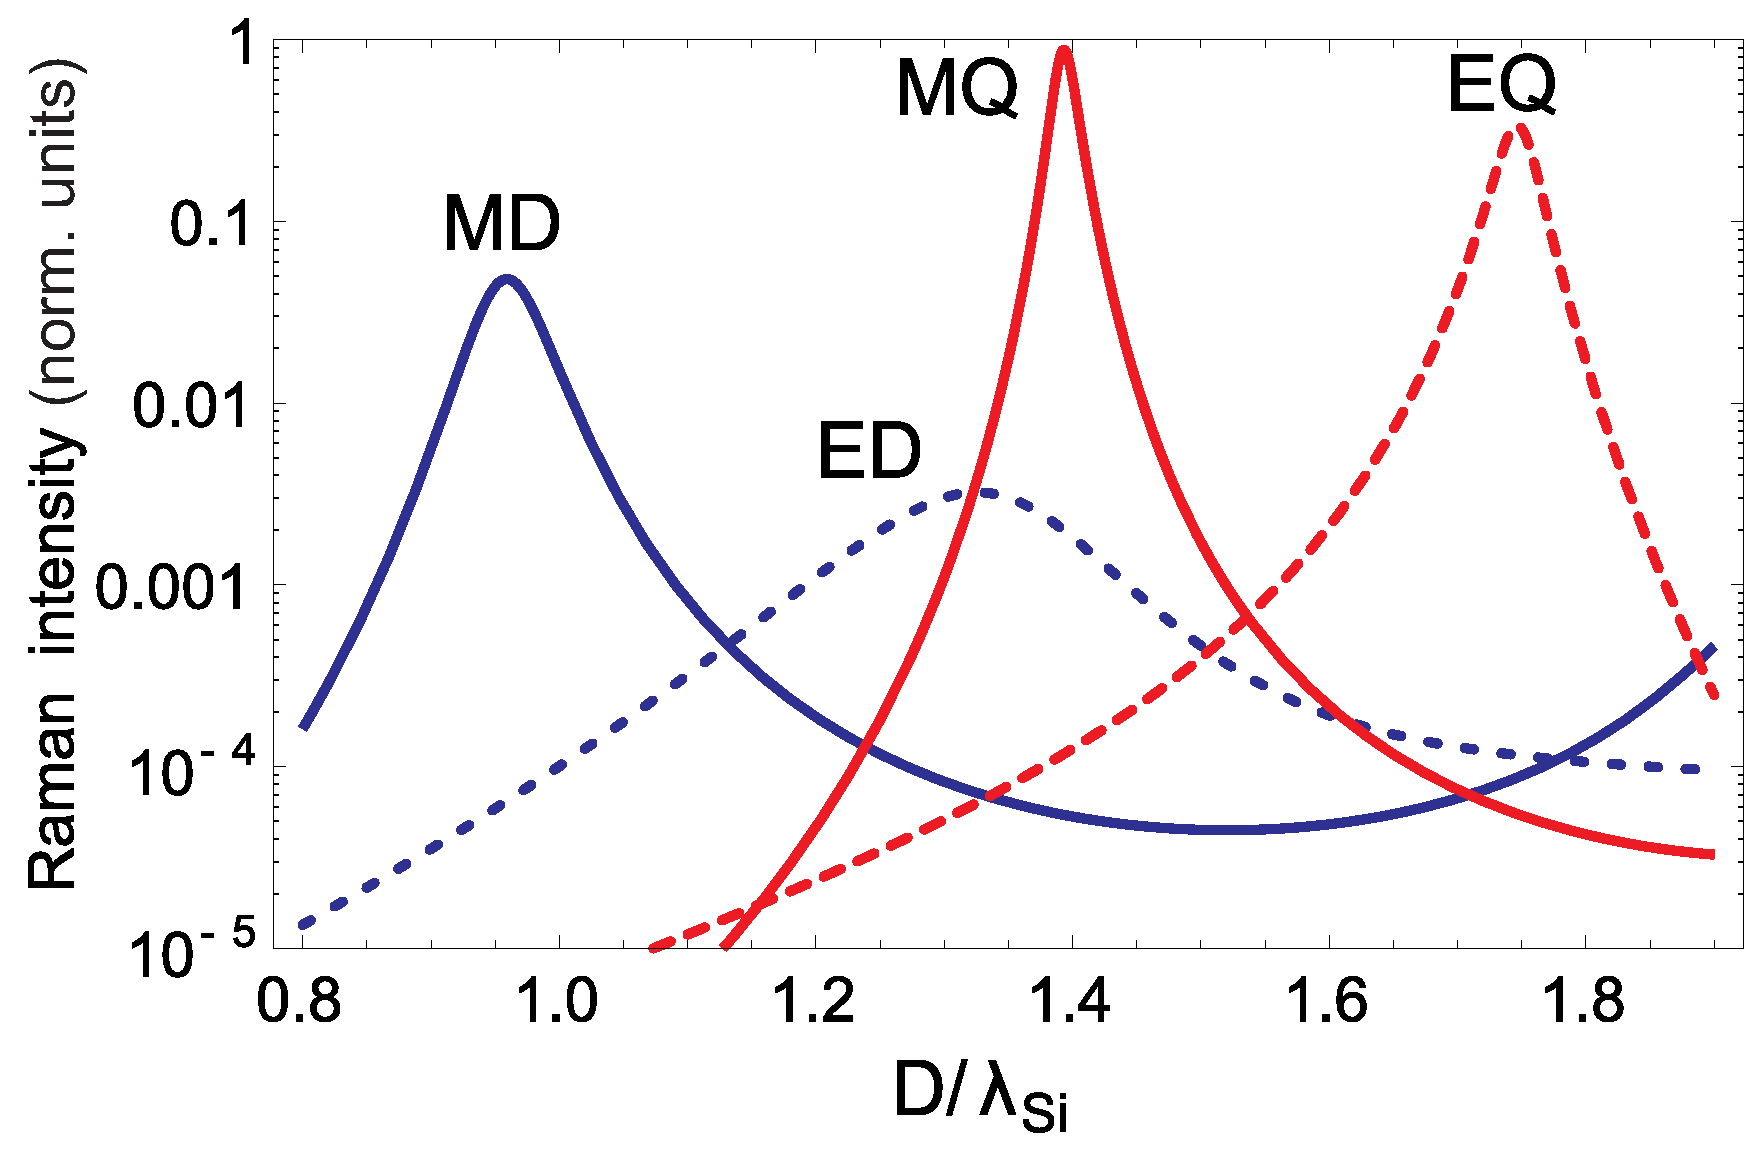
\includegraphics[width=0.5\textwidth]{figs/intro/TheoryEnhancement.eps}
            \end{center}
            \caption{Log plot of normalized intensity of Raman scattering as a function of dimensionless nanoparticle diameter for the magnetic dipole (MD),
            electric dipole (ED), magnetic quadrupole (MQ) and electric quadrupole (EQ) resonances.}
            \label{fig:TheoryEnhancement}
        \end{figure}

            Expression~(\ref{eq5}) can be simplified with the use of the single-mode approximation. First, we notice that the
        electromagnetic response of an optically small Si nanoparticle at the excitation wavelength is dominated by a single
        magnetic or electric multipole resonance depending on the particle radius~\cite{evlyukhin2010optical}. Therefore, we can keep
        only one resonant term in Eq.~(\ref{eq1}) and represent the electric field inside the nanoparticle as ${
        {\mathbf{{E}}}_{exc}} \approx {E_n}{c_n}{\mathbf{M}}_{o1n}^{(1)}$, for the $n-$th magnetic resonance, and
        ${{\mathbf{{E}}}_{exc}}\approx -i{E_n}{d_n}{\mathbf{N}}_{e1n}^{(1)}$, for the $n-$th electric resonance,
        respectively. Furthermore, since the Raman shift in silicon is small compared to the linewidth $\gamma$ of
        Mie resonance at $\omega_0$, the main contribution to the Green tensor is provided by the same eigenmode of
        the system. Therefore, expanding the Green tensor in the series of eigenmodes~\cite{ishimaru1991electromagnetic} and keeping only
        the resonant term, we obtain
        %
        \begin{align}
            {\hat G_s}\left( {{{\bf{r}}_0},{\bf{r}}} \right) \approx \frac{{{c^2}}}{{{N^2}}}\frac{{{\bf{u}}\left( {{{\bf{r}}_0}} \right) \otimes
            {\bf{u}}^*\left( {\bf{r}} \right)}}{{{{\left( {{\omega _0} + i\gamma } \right)}^2} - \omega _s^2}},
            \label{eq8}
        \end{align}
        %
        where ${{\mathbf{u}}\left( {{\mathbf r}} \right)}$ is the spatial field distribution of the eigenmode, and
        ${N^2} = {\int {{\mathop{\rm Re}\nolimits} \varepsilon \left( {\bf{r}} \right)\left| {{\bf{u}}\left( {\bf{r}} \right)} \right|} ^2}{d^3}{\bf{r}}$
        is the normalization constant. Finally, integrating the expression (5) over the whole volume $V$ of the nanoparticle, we
        arrive at the following simple expression describing the Raman signal enhanced by a single Mie resonance:
        %
        \begin{align}
            S\left( {{{\mathbf{r}}_0}} \right) \approx V{\left( {\frac{{{\omega _s}}}{c}} \right)^4}{\left| {\frac{{{\chi_s s_n}}}{{{{\left( {{\omega
            _0} + i\gamma } \right)}^2} - \omega _s^2}}} \right|^2},
            \label{eq9}
        \end{align}
        %
        where $s_n$ stands for the Mie coefficient, either $c_n$ or $d_n$ of the corresponding mode. The above expression clearly
        shows that the total enhancement of Raman scattering depends on two factors: the enhancement of the excitation field
        inside the medium, and the Purcell enhancement of the Raman dipoles radiation~\cite{checoury2010deterministic}.

        The two key parameters entering Eq.~(\ref{eq9}) are the resonance frequency $\omega_0$ and the resonance linewidth $\gamma$.
        The resonance frequency can be easily estimated numerically, while for the estimation of the resonance linewidth one can
        employ analytical expressions from Ref.~\cite{lai1991effect}. Substituting these values into Eq.~(\ref{eq9}), we obtain the desired
        spectrum of Raman scattering enhanced by the resonances of a silicon sphere. This spectrum (normalized by the particle
        volume $V=4\pi R^3/3$) is plotted in Fig.~\ref{fig:TheoryEnhancement} as a  function of dimensionless nanoparticle diameter $D/\lambda_{\rm Si}$
        with $\lambda_{\rm Si}=163$~nm being the wavelength of the excitation signal inside the silicon for the magnetic dipole (MD), electric dipole (ED),
        magnetic quadrupole (MQ) and electric quadrupole (EQ) resonances assuming a constant excitation wavelength of 633~nm,
        used below in experiments.

        The derived single-mode expression (\ref{eq9}) allows us to clearly separate contributions of each Mie resonance of the
        nanoparticle into the total Raman scattering enhancement. As follows from Fig.~(\ref{fig:TheoryEnhancement}), the strongest enhancement
        is associated with the MQ resonance due to its high $Q-$factor. Notably, the predicted Raman scattering enhancement
        at the MD resonance, which occurs for the smallest particles, is more than an order of magnitude larger than that for
        the ED resonance.


    \subsubsection{Numerical Methods}
    \label{sec:Numeric}
        Several numerical methods were used to simulate the scattering properties of the fabricated nanoparticles~--- to prove their
        crystalline phase, to probe their shape, to determine their size. The initial idea was to use the Discrete Dipole Approximation,
        because it is very flexible and can work with scatterers of arbitrary geometry. The main problem we encountered was the fact
        the method is very involved (especially if one tries to incorporate substrate interaction), and computationally intensive for
        the required problems. Many calculations turned out to be excessive~-- a simple Mie theory calculation,
        while simulating the incorrect geometry, was more than enough to model the required parameters, with error well within the
        requirements.

        For calculations of field distribution inside the nanoparticles presented in this thesis, CST Microwave Studio was used.
        It is an  EM simulation package that uses the Finite Integration Technique for most of its calculations.

        \subsubsection{Discrete Dipole Approximation}
        \label{subsec:DDA}

                For the DDA calculations, a custom, Python-based implementation was written, PyDDA~--- a reimplementation of an existing
            Matlab toolkit, DDA-SI\cite{loke2011discrete}. The implementation even included surface-interaction components in its' calculations,
            but the complexity of the calculation and difficulty of accurately modeling particles led to the DDA being abandoned in favor of plain
            Mie theory, which provided more than enough accuracy for the purposes of the project.

            \begin{figure}[h!]
                \centering
                \begin{subfigure}[b]{0.3\textwidth}
                    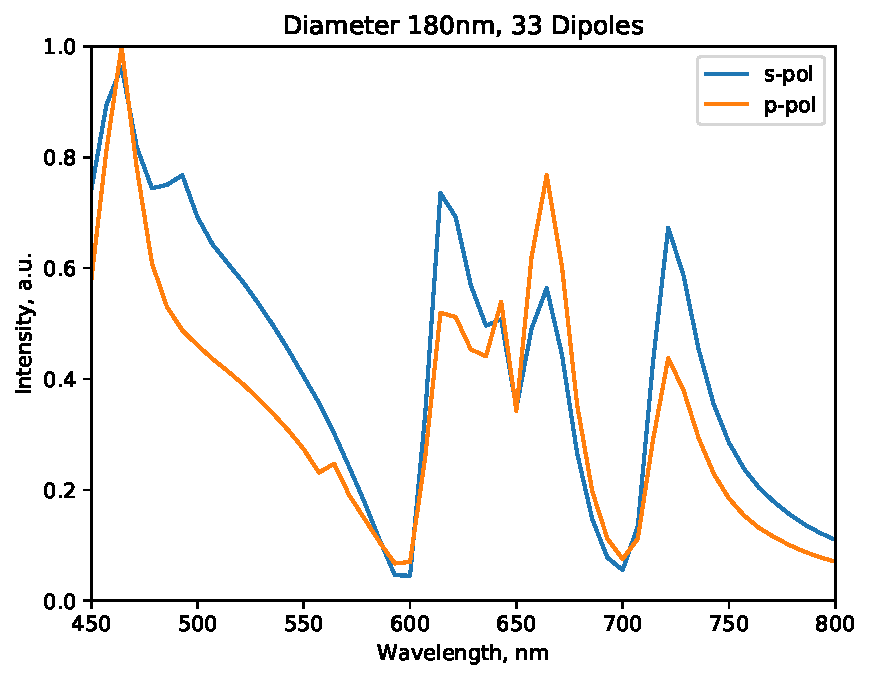
\includegraphics[width=\textwidth]{figs/methods/DDA/n_33.pdf}
                    \caption{}
                \end{subfigure}~
                \begin{subfigure}[b]{0.3\textwidth}
                    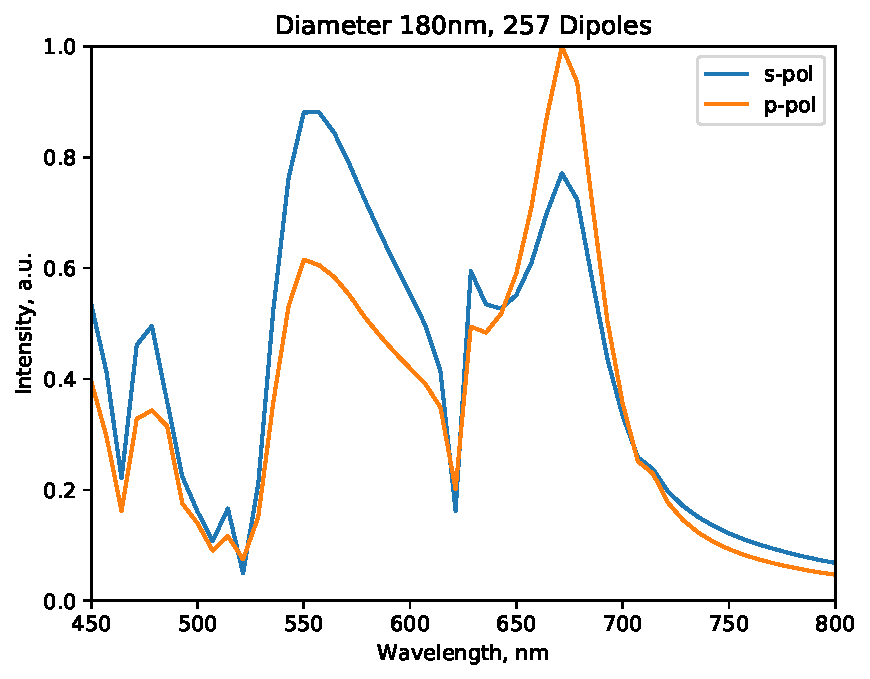
\includegraphics[width=\textwidth]{figs/methods/DDA/n_257.pdf}
                    \caption{}
                \end{subfigure}~
                \begin{subfigure}[b]{0.3\textwidth}
                    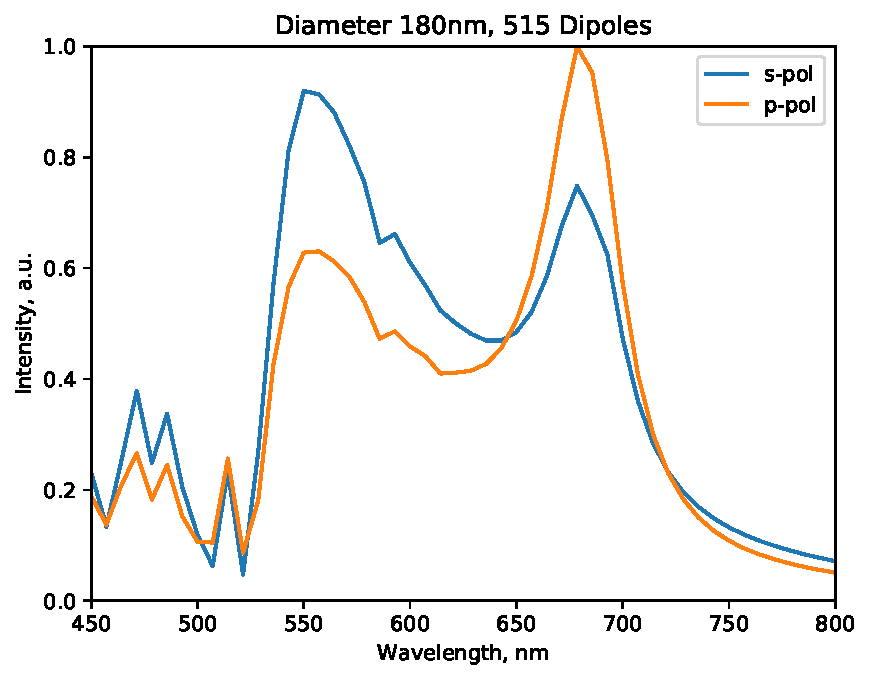
\includegraphics[width=\textwidth]{figs/methods/DDA/n_515.pdf}
                    \caption{}
                \end{subfigure}
                \caption{Scattering from isotropic sphere modeled by DDA using a) 33, b) 257, c) 515 dipoles to model the sphere.}
                \label{fig:DDA_Dipole}
            \end{figure}

        \clearpage
        \subsubsection{Finite Integration Technique}
        \label{subsec:FIT}

                CST Microwave studio was used to model field distribution inside and around the silicon nanoparticles, to
            demonstrate the electric field confinement at different types of resonances (electric and magnetic dipole resonances).
            The model was a slightly oblate spheroid, corresponding to the experimentally determined geometric parameters of the
            nanoparticles.

            \begin{figure}[!ht]
                \centering
                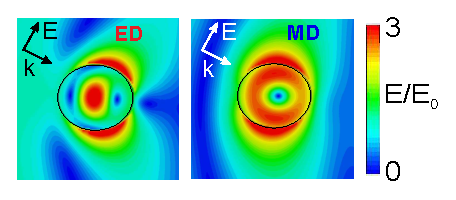
\includegraphics[width=0.7\textwidth]{figs/methods/FIT/CST.eps}
                \caption{Field distribution inside 180nm spheroid nanoparticle with 1.12 oblateness parameter at electric and magnetic dipole resonances,
                    calculated using CST Microwave Studio}
                \label{fig:CST}
            \end{figure}

\clearpage
